\chapter{Basic concepts}
\label{chapter:epipilar_geo}

\section{Homogenous coordinate system}

In projective geometry, the homogenous coordinate system is used in the same way as Cartesian coordinates are in Euclidean geometry.
To transform a point $x=(u, v)^T$ from cartesian coordinates to homogenous, simply append $1$ as the third coordinate: $x=(u, v, 1)^T$.
Homogenous coordinates are used to simplify the 2D transformation operations:

\begin{center}
    \textbf{Scale}
\end{center}
$$
\begin{bmatrix}
    x_1 \\ y_1
\end{bmatrix} = 
\begin{bmatrix}
    s_x & 0 \\
    0 & s_y
\end{bmatrix}
\begin{bmatrix}
    x_0 \\ y_0
\end{bmatrix}
$$ 
\begin{center}
    \textbf{Rotation}    
\end{center}
$$
\begin{bmatrix}
    x_1 \\ y_1
\end{bmatrix} = 
\begin{bmatrix}
    cos(\theta) & -sin(\theta) \\
    sin(\theta) & cos(\theta)
\end{bmatrix}
\begin{bmatrix}
    x_0 \\ y_0
\end{bmatrix}
$$
\begin{center}
    \textbf{Translation}    
\end{center}
$$
\begin{bmatrix}
    x_1 \\ y_1
\end{bmatrix} = 
\begin{bmatrix}
    x_0 \\ y_0
\end{bmatrix} +
\begin{bmatrix}
    t_x \\ t_y
\end{bmatrix}
$$ 

To apply any transformation, it is required to make a sequence of matrix multiplications, but this is not the case with translation - an addition operation is needed for that. Here are these operation in projective geometry:

\begin{center}
    \textbf{Scale}
\end{center}
$$
\begin{bmatrix}
    x_1 \\ y_1 \\ 1
\end{bmatrix} = 
\begin{bmatrix}
    s_x & 0 & 0\\
    0 & s_y & 0\\
    0 & 0 & 1
\end{bmatrix}
\begin{bmatrix}
    x_0 \\ y_0 \\ 1
\end{bmatrix}
$$ 
\begin{center}
    \textbf{Rotation}    
\end{center}
$$
\begin{bmatrix}
    x_1 \\ y_1 \\ 1
\end{bmatrix} = 
\begin{bmatrix}
    cos(\theta) & -sin(\theta) & 0 \\
    sin(\theta) & cos(\theta)  & 0 \\
    0 & 0 & 1
\end{bmatrix}
\begin{bmatrix}
    x_0 \\ y_0 \\ 1
\end{bmatrix}
$$
\begin{center}
    \textbf{Translation}    
\end{center}
$$
\begin{bmatrix}
    x_1 \\ y_1 \\ 1
\end{bmatrix} = 
\begin{bmatrix}
    1 & 0 & t_x\\
    0 & 1 & t_y\\
    0 & 0 & 1
\end{bmatrix}
\begin{bmatrix}
    x_0 \\ y_0 \\ 1
\end{bmatrix}
$$ 

So in the homogenous coordinate system, all 2d transformations can be combined and expressed as matrix multiplications.

\subsection{Infinity}
\begin{figure}[h]
    \centering
    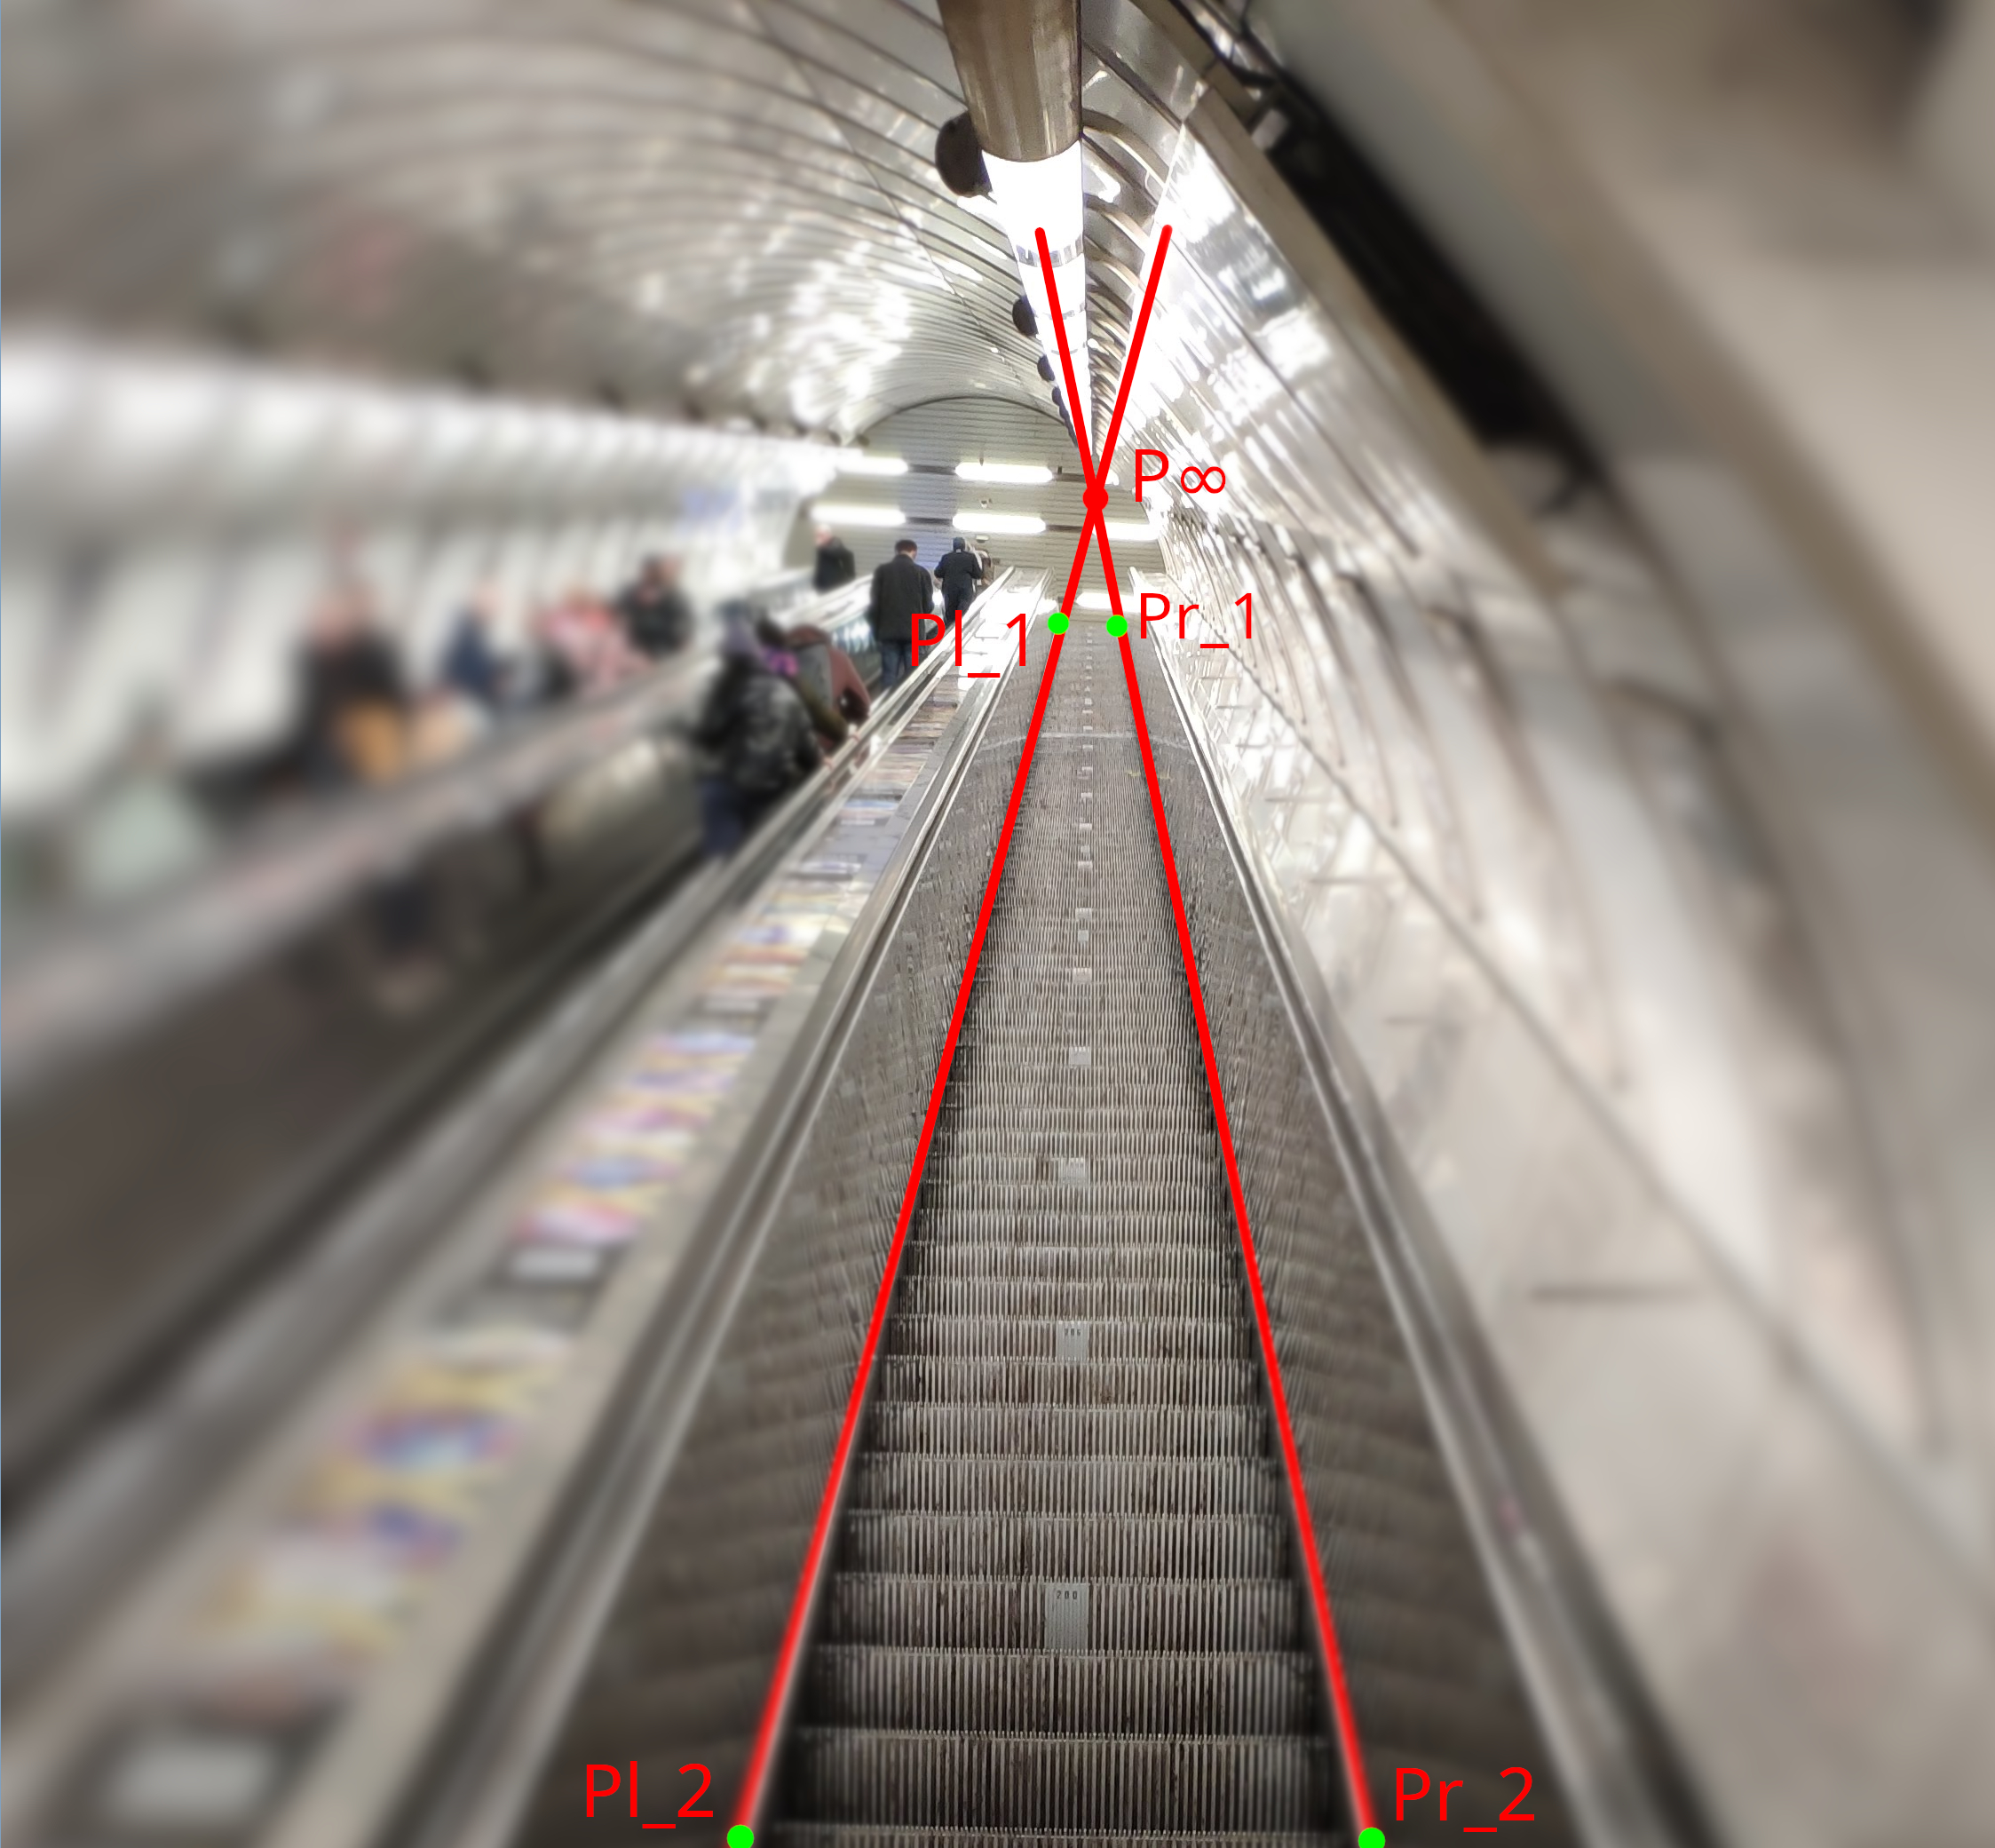
\includegraphics[width=0.7\textwidth]{graphics/parallel_intersection.jpg}
    \caption{Parallel lines intersection}
    \label{fig:intersection_parallel}
\end{figure}

\begin{figure}[h]
    \centering
    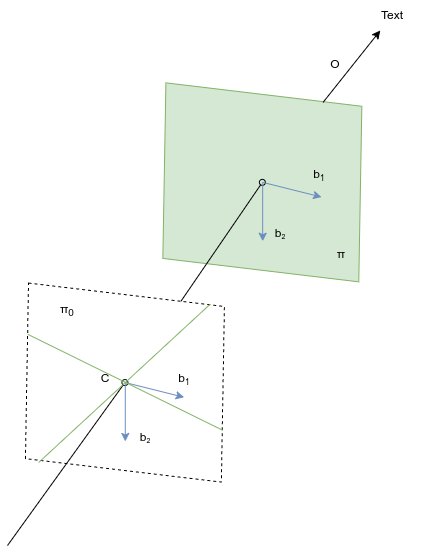
\includegraphics[width=.5\textwidth]{graphics/homogenous.png}
    \caption{Scheme of homogenous coordinates}
    \label{fig:homogenous}
\end{figure}

In Euclidian geometry, parallel lines are the lines that have no intersection point. 
In projective geometry, parallel lines intersect at a point $x$ at infinity. 
How is it possible? 
In the image \autoref{fig:intersection_parallel} let $l_r = Pr_1 \cap Pr_2 $ and $l_l = Pl_1 \cap Pl_2$. 
In the 3D world, we know that lines $l_l \parallel l_r$, but after projection on the image plane $\Pi$, we can calculate - in this case even see - the intersecting point $P_{\infty}$. 

Both line and point in a homogenous coordinates can be expressed as vector of three numbers, but if in case of a point homogenous $x = (x, y, z)^T$ will be $m = (\frac{x}{z}, \frac{y}{z})^T$, line $l = (a, b, c)^T$, where $a, b, c$ are parameters of a line equation $ax + by + c = 0$. 
In general case point at infinity is called an \textit{ideal point} and it is not seen on the image, it's coordinates can be expressed as $x_{\infty} = (u, v, 0)^T, \{u, v\} \neq 0$. Same about line - such line is called \textit{ideal line} and it's coordinates are $l = (0, 0, c), c \neq 0$. In algebraic representation, both ideal point and line are lying at the plane $\Pi_0$ (\autoref{fig:homogenous}, green lines).

\section{Pinhole camera model}
A pinhole camera - or a canonical perspective camera model - is a model of a simple camera without optics.
The first example is a camera obscura - a dark room with a small hole through which the image from outside is projected on the opposite wall. 
This model can be used to express camera geometry with a field of view angles less than $180^{\circ}$.

\subsection{Camera coordinate system}
\begin{figure}[h]
    \centering
    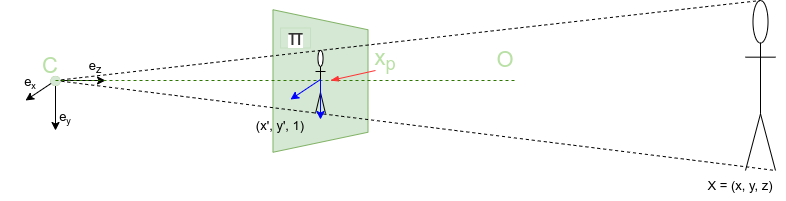
\includegraphics[width=1\textwidth]{graphics/td_scene.png}
    \caption{The pinhole camera model working scheme}
    \label{fig:td_scene_3d}
\end{figure}

\begin{figure}[h]
    \centering
    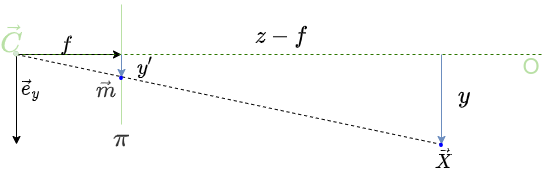
\includegraphics[width=0.9\textwidth]{graphics/td_scene_yz.png}
    \caption{The pinhole camera model, y-z plane}
    \label{fig:td_scene_yz}
\end{figure}

\begin{figure}[h]
    \centering
    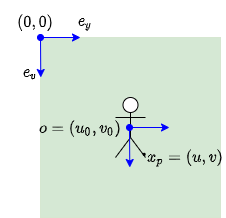
\includegraphics[width=.4\textwidth]{graphics/td_scene_xy.png}
    \caption{The pinhole camera model, x-y plane}
    \label{fig:td_scene_xy}
\end{figure}

In the physical implementation of the Obscure camera, the projective plane is on the opposite side from the Projection centre (or Camera centre $C$ in the pinhole camera model), the image is reversed and mirrored, but in most computer vision literature, authors assume that it is on the same side as an object (see \autoref{fig:td_scene_3d}).
In \autoref{fig:td_scene_3d} we are looking through a camera with camera center $C$ in a coordinate system with origin at $C$ and basis vectors $(e_x, e_y, e_z)$ on a human. 
Each point $X = (x, y, z)^T$ in a world coordinate system has it's projection $x_p = (x', y', 1)^T$ on a plane $\Pi$ which is located on a distance 1 from a camera center (\autoref{fig:td_scene_yz}). 
Optical axis $O$ is a ray perpendicular to plane $\Pi$, and on the image the point $ O \cap \Pi = x_p$ is a center of the image, see \autoref{fig:td_scene_xy}).

\subsection{Camera calibration matrix}
\begin{figure}[h]
    \centering
    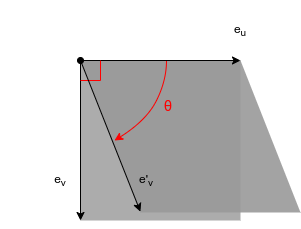
\includegraphics[width=.6\textwidth]{graphics/pixel.png}
    \caption{Scheme of pixel, changing the image (inner) reference frame}
    \label{fig:Kframes}
\end{figure}
Camera calibration matrix - a matrix that includes camera \textit{intrinsic} parameters - pixel size ($e_u$ and $e_v$) and pixel skew angle ($\theta$), as on \autoref{fig:Kframes}, pixel aspect ratio $\bf{a}$ and principle point coordinates $x_p = (u_0, v_0)$.
$$
K = \begin{bmatrix}
    af & -a f cot(\theta) & u_0 \\
    0 & f / sin(\theta) & v_0 \\
    0 & 0 & 1 \\
\end{bmatrix} \hspace{1cm} units: [f]=px, [u_0]=px, [v_0]=px, [a]=1
$$ 
Where $f$ is a focal length used to convert world length ratios to pixels.

In the modern world, every digital camera has a calibration matrix with a square pixel, so in most cases, the camera matrix looks like this:

$$
K = \begin{bmatrix}
    f & 0 & u_0 \\
    0 & f & v_0 \\
    0 & 0 & 1 \\
\end{bmatrix}
$$

\subsection{Projection matrix}

\begin{figure}[h]
    \centering
    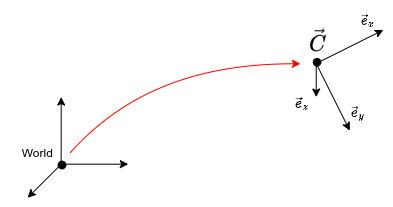
\includegraphics[width=.5\textwidth]{graphics/frames.png}
    \caption{Changing the world (outer) reference frame}
    \label{fig:frames}
\end{figure}
To translate a point from a world coordinate frame to an image coordinate frame, the Image projection matrix $P$ is used. 
The canonical projection matrix $P_0$ assumes that the camera is in the world coordinate centre and that the calibration matrix $K = \bf{I}$
$$
P_0 = \begin{bmatrix} \bf{I} & | & 0 \end{bmatrix} = 
    \begin{bmatrix}
    1 & 0 & 0 & 0 \\
    0 & 1 & 0 & 0 \\
    0 & 0 & 1 & 0 \\
    \end{bmatrix}
$$
However, this case is degenerate. 
As far as each camera is different, the canonical projection matrix is never used. Instead, image projection matrix $P$ is used, with applied calibration matrix $K$ to transform canonical $P_0$ to perspective $P$:

$$
P = \bf{K} \begin{bmatrix} \bf{I} & | & 0 \end{bmatrix} = 
    \begin{bmatrix} 
    f & 0 & u_0 & 0 \\
    0 & f & v_0 & 0 \\ 
    0 & 0 & 1 & 0 \\
    \end{bmatrix}
$$

However, not always; the world coordinate centre is located at point $C$ \autoref{fig:frames}. 
Usually it is rotated using a rotation matrix $R$ and translated on vector $t$ where $R$ is a $3x3$ matrix with $det(R) = 1$ and $R^{-1} = R^T$. 
So, in the general case:

$$
P =   K \begin{bmatrix} \bf{R} & | & \vec{\bf{t}} \end{bmatrix} = 
        K \begin{bmatrix} \bf{R} & | & - \bf{R} \bf{C} \end{bmatrix}
$$
where $C$ is often used as a camera position in a world reference frame. 
So matrix $P$ have six intrinsic parameters: 3 Euler angles and three translation components. 

\subsection{Projection equation}

Image point $m = (u, v)^T$ can be obtained from a point $X$ using $P$ 

$$
\lambda \begin{bmatrix} 
    u \\ v \\ 1 \end{bmatrix} = P \begin{bmatrix} x \\ y \\ z \\ 1
\end{bmatrix}
$$
$$
\lambda \begin{bmatrix} 
    \vec{m} \\ 1 \end{bmatrix} = P \begin{bmatrix} \vec{X} \\ 1
    \end{bmatrix}
$$
Where $\lambda \neq 0$

\section{Epipolar geometry}

\subsection{Skew-symmetric 3x3 matrix}
From \cite{hartley_zisserman_2004}, p.581.


Skew-symmetric or antisymetric matrix is such matrix $[b]_{\times}$ that $[b]_{\times}^T = -[b]_{\times}$. 
For vector $b = (b_1, b_2, b_3)^T$:

$$
[b]_{\times} = \begin{bmatrix}
    0 & -b_3 & b_2 \\ 
    b_3 & 0 & b_1 \\ 
    -b_2 & b_1 & 0 \\ 
\end{bmatrix}
$$
This matrix has some essential properties, but the most important in this thesis - it generalizes across a product as matrix multiplication.
$$
a \times b = [a]_{\times} b
$$

\subsection{Epipolar geometry}
\begin{figure}[h]
    \centering
    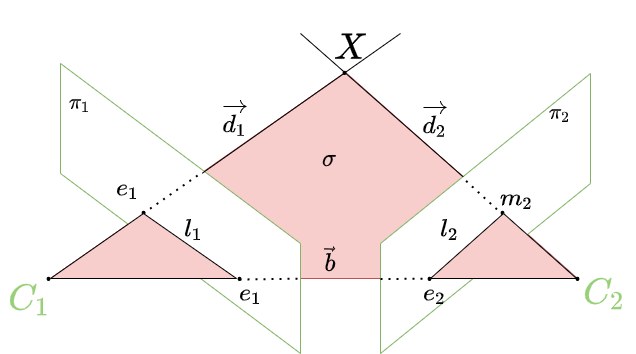
\includegraphics[width=1\textwidth]{graphics/epipolar.png}
    \caption{Epipolar geometry scheme}
    \label{fig:epipolar_std}
\end{figure}
\autoref{fig:epipolar_std} shows a scheme of two cameras with different camera centers $C_1$ and $C_2$ connected with a base line $b = C_2 - C_1$. 
Both of them are seen as some 3d point $X$. 
This point projections are $m_1$ and $m_2$ respectivly. 
Points $C_1, C_2$ and $X$ form an \textit{epipolar plane} $\sigma$.
$\sigma \cap \pi_1 = l_1$ and $\sigma \cap \pi_2 = l_2$ are images of \textit{epipolar lines}. 
Epipolar line $l_1$ passes through \textit{epipole} $e_1$, where $\lambda [e_1 | 1]^T = P_2 C_1$, respectivly $\lambda [e_2 | 1]^T = P_1 C_2$.

\subsection{Epipolar constraint}
Having a set of two cameras the relationship between them and constraints on them can be expressed by two new matrices: 
\textit{Essential matrix} $E \in \mathbb{R}^{3x3}, rank(E) = 2$
$$
E = R_2 [C_2 - C_1]_{\times} R_1^T = [-t_{21}]_{\times}R_{21}
$$ 
and \textit{Fundamental matrix} $F \in \mathbb{R}^{3x3}, rank(F) = 2$
$$
F = K_2^{-T} R_2 [C_2 - C_1]_{\times} R_1^T K_1^{-1} = K_2^{-T} [-t_{21}]_{\times} R_{21} K_1^{-1} = K_2^{-T} E K_1^{-1}
$$
where 
$R_{21} = R_2 R_1^T$ is a relative camera rotation and 
$t_{21} = -R_2 b = t_2 - R_{21}t_1$ is a relative camera translation.
The translation $t_{21}$ is lost since E is homogenous.
Epipolar constraint looks like
$$
\begin{bmatrix} m_2 & | & 1 \end{bmatrix} F \begin{bmatrix} m_1 \\ 1 \end{bmatrix} = 0
$$
$F$ maps point to lines, such as
$$
\lambda l_1 = F^T \begin{bmatrix} m_2 \\ 1 \end{bmatrix}
$$
$$
\lambda l_2 = F \begin{bmatrix} m_1 \\ 1 \end{bmatrix}
$$
Also, some other properties of the $F$ matrix:
$$
F \begin{bmatrix} e_1 \\ 1 \end{bmatrix} = F^T \begin{bmatrix} e_2 \\ 1 \end{bmatrix} = 0
$$
